\documentclass[12pt]{article}

\usepackage{geometry}
 \geometry{
 a4paper,
 left=25mm,
 right=20mm,
 top=20mm,
 }
 
\usepackage{hyperref}
\usepackage{exercise}
\usepackage{enumerate}
\usepackage{graphicx}
\usepackage{subfig}
\usepackage{listings}
\usepackage{tikz}

\usepackage{amsmath}
\usepackage{amsfonts}

\usetikzlibrary[topaths]

\renewcommand{\baselinestretch}{1.2}

%\usepackage[active,tightpage]{preview}

%\PreviewEnvironment{tikzpicture}
%\setlength\PreviewBorder{5pt}

\newcommand\MyFive[2]{%
  \foreach \x in {1,...,5}{
    \pgfmathparse{(\x-1)*72+floor(\x/6)*36 + 90 - 90*#2}
    \node[draw,circle,inner sep=5pt,text width=1cm, align=center] (#1-\x) at (\pgfmathresult:2.5cm){ \ifthenelse{1 = \x}{Master Node}{Node $\x$}};
  }
  \foreach \x [count=\xi from 1] in {1,...,5}{
    \foreach \y in {\x,...,5}{
    \path (#1-\xi) edge[-] (#1-\y);
  }
}
}


\lstset{language=erlang, firstline=37, lastline=45, title={Listing 1: Data structures for cellular automaton}}

\begin{document}

\title{
Distributed Systems \\
\textbf{Building a Middleware for Distributed System in Erlang}\\
Project report
}

\author{Ievgeniia Oshurko}
\date{April 16, 2016}
\maketitle


\section{Introduction}

In this project a middleware for distributed system was implemented. The main function of the middleware is to manage cluster consisting of connected remote nodes. This cluster can be used for handling big load of small tasks. 

\textbf{Topology}. The remote nodes are connected into clique topology forming a fully connected network so that all nodes have direct links to other nodes. \emph{Why clique topology has been chosen?} Clique topology has an overhead in the number of  connection links, but at the same time it is highly fault tolerant. In case of crash of any node in the network, its topology does not change, and all nodes stay connected. Consider the performance requirements for our distributed system: we want a huge number of incoming small jobs to be distributed into our system efficiently. As master node has direct link to each node, it takes exactly one hop for master to send a message to any node. 

\begin{center}
	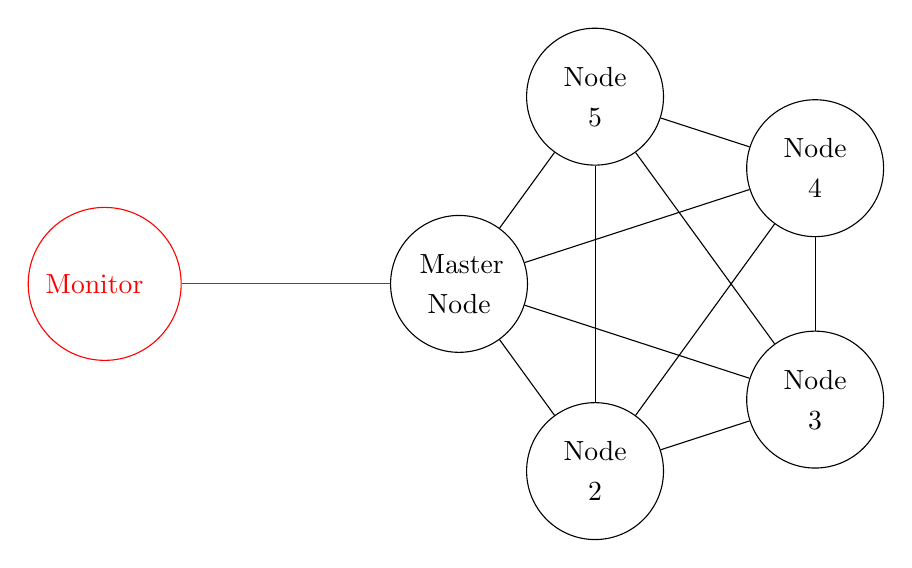
\begin{tikzpicture}
		\node[draw,circle,inner sep=5pt,text width=1.5cm,color=red](Monitor1){ Monitor };
		\begin{scope}[xshift=7cm]
		 \MyFive{A}{-1}
		\end{scope}
		\draw[red] (Monitor1) -- (A-1);
	\end{tikzpicture}
	
	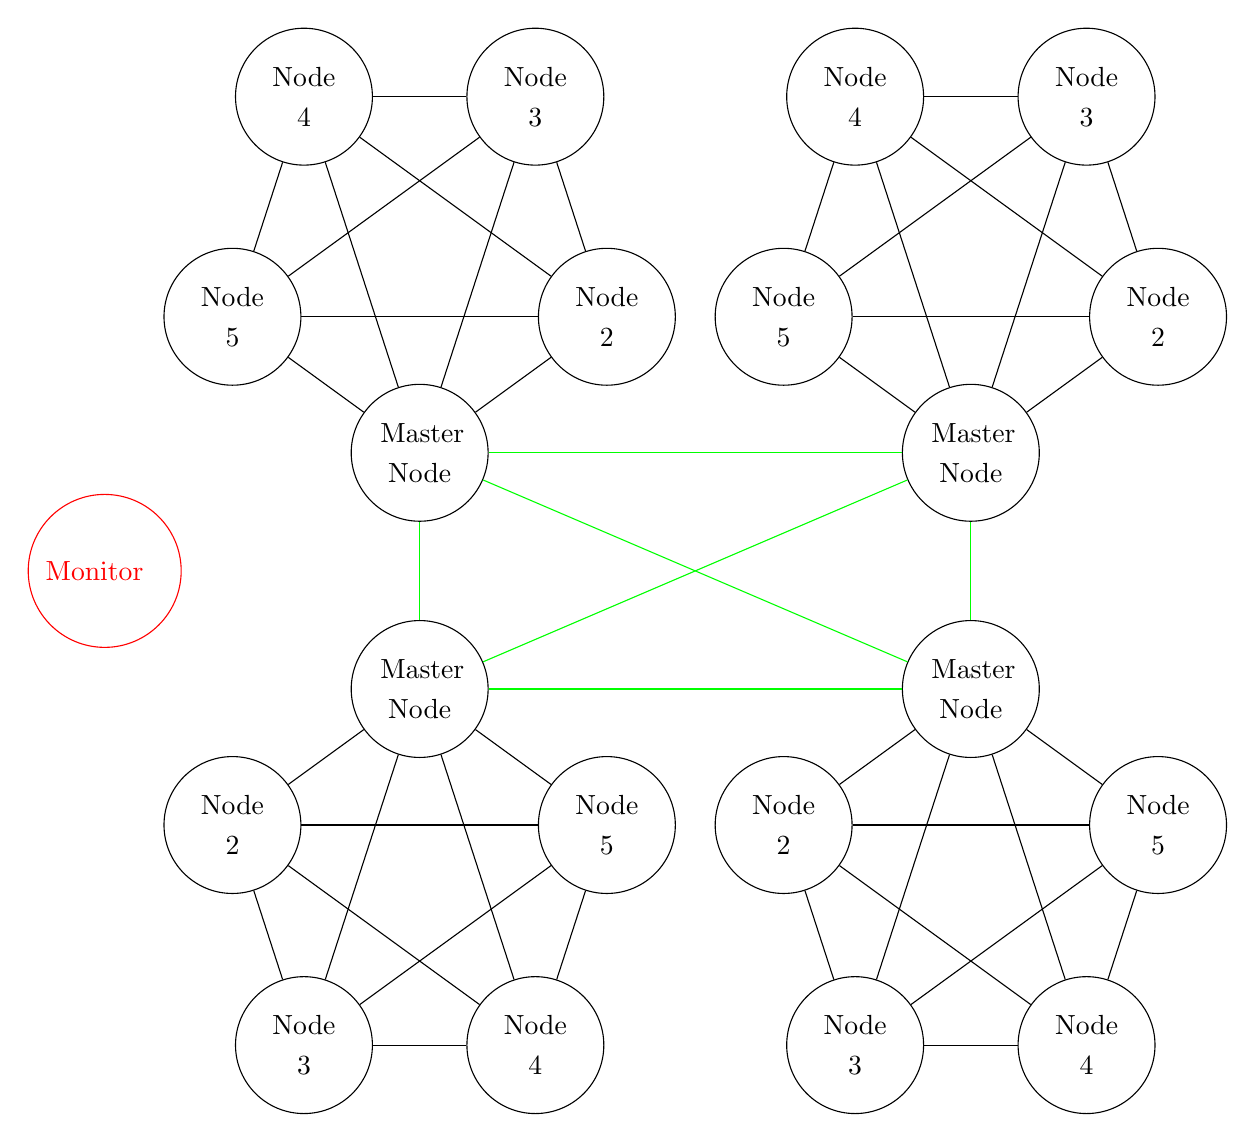
\begin{tikzpicture}
		\MyFive{B}{2}
		\begin{scope}[xshift=7cm]
		 \MyFive{C}{2}
		\end{scope}
		\begin{scope}[xshift=-4cm, yshift=-4cm]
		\node[draw,circle,inner sep=5pt,text width=1.5cm,color=red](Monitor1){ Monitor };
		\end{scope}
		\begin{scope}[yshift=-8cm]
		 \MyFive{D}{0}
		\end{scope}
		\begin{scope}[xshift=7cm, yshift=-8cm]
		 \MyFive{E}{0}
		\end{scope}
		\draw[green] (B-1) -- (C-1);
		\draw[green] (D-1) -- (E-1);
		\draw[green] (B-1) -- (D-1);
		\draw[green] (C-1) -- (E-1);
		\draw[green] (B-1) -- (E-1);
		\draw[green] (D-1) -- (C-1);
	\end{tikzpicture}
	
\end{center}
\textbf{Structure}.

Implemented module consists of two submodules: \texttt{agents.erl} and \texttt{monitor.erl}

Fault tolerant

\section{Agent deployment}
\subsection{Start/stop a cluster}
\subsection{Adding the nodes}
\subsection{Removing the nodes}
\subsection{Cluster scaling}
\section{Remote job execution}
\subsection{Distribution of jobs}
\subsection{Node removal}
\section{Agent monitoring}
\subsection{Nodes alive}
\subsection{Death of master node}
\section{Examples and applications}

Couple of examples where implemented. Script that deploy the middleware on the nodes, so they are ready to recieve the job.

Application: there is no distribution on task level - so each task is executed by a single node. The system is suitable for application where the number of incoming tasks, as it distributes them equally between the nodes. Smth like Web-server with numberous request from clients.


\end{document}
